\documentclass[11pt,a4paper]{article}

\newcommand{\tumsoTime}{09:00 น. - 12:00 น.}
\newcommand{\tumsoRound}{1}

\usepackage{../tumso}

\begin{document}

\begin{problem}{SPL Simple Potato Language}{standard input}{standard output}{0.5 seconds}{64 megabytes}{75}

มีการคิดค้นเครื่องคำนวณสุดทรงพลังขึ้นมาชื่อ Potato Model A และได้มีการออกแบบภาษาโปรแกรมที่ชื่อว่า SPL ขึ้นมาแต่เนื่องจากการขอเข้า Access เครื่อง Potato Model A นั้นยากมากๆจึงเป็นการยากที่เราจะได้ลองเขียนภาษา SPL กระทรวงกลาโหมจึงได้มอบหมายให้น้องเขียน Compiler/Interpeter สำหรับภาษา SPL เพื่อให้นักวิจัยของทางกองทัพได้ฝึกภาษา SPL ในการพัฒนาอาวุธสำหรับกำจัดแมลงสาปออกจากห้องทำงานของ นายก

\begin{figure}[htp]
\centering
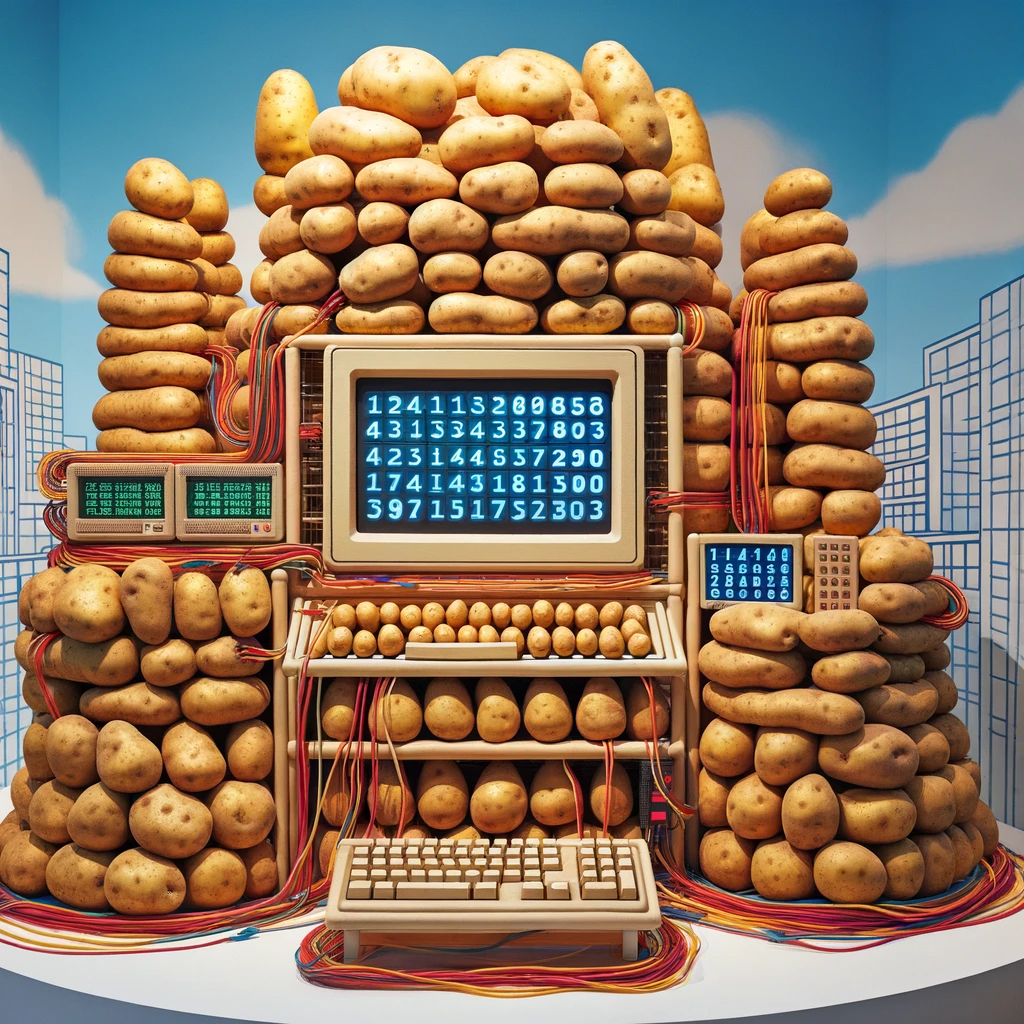
\includegraphics[width=6cm]{simplepotatolanguage/Potato Model A.png}
\caption{เครื่อง Potato Model A}
\end{figure}

\newpage

โดยภาษา SPL นั้นมีความเรียบง่ายและทำงานบน Stack-based architecture หรือคือใช้ stack data structure สำหรับเก็บข้อมูลและประมวลผลโดย SPL มีลักษณะต่อไปนี้
\begin{enumerate}
    \item ลักษณะของ Potato Stack
    \begin{itemize}
        \item Potato Stack เป็น A last-in, first-out (LIFO) เข้าหลังออกก่อน
        \item Potato Stack สามารถทำ Operation ต่างๆได้เช่น PUSH POP
        \begin{figure}[htp]
        \centering
        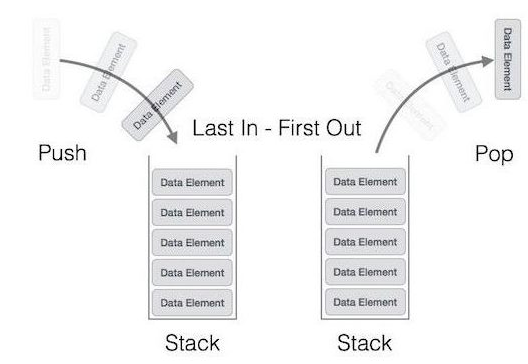
\includegraphics[width=6cm]{simplepotatolanguage/LIFO.png}
        \caption{ลักษณะ LIFO ของ Potato Stack}
        \end{figure}
    \end{itemize}
    
    \item เนื่องจาก Potato Model A พัฒนา CPU ด้วย Potato Architecture และเก็บตัวเลขเป็นจำนวนมันฝรั่งจึงเก็บข้อมูลได้เป็น Unsigned 8-bit integer เท่านั้นค่าที่ออกนอก range 0-255 จะ Overflow หรือ Underflow เช่น -1 = 255, 257 = 1 ทศนิยมจะโดนปัดลงเสมอ
    \item เครื่อง Potato Model A มี Instruction Set จำกัดดังนี้
    \begin{itemize}
        \item \verb|PUSH (T)| : นำข้อมูลใส่เข้าไปยัง Potato Stack เช่น T5T4 Potato Stack จะมีข้อมูลดังนี้ หัว-4-5-ท้าย
        \item \verb|POP (P)| : นำข้อมูลออกจาก Potato Stack เช่น PP นำข้อมูล 2 ตัวบนออกจาก Potato Stack
        \item \verb|ADD (A)| : นำข้อมูล 2 ตัวบนออกจาก Potato Stack หาผลบวกแล้ว PUSH เข้าไปใน Potato Stack
        \item \verb|SUB (S)| : นำข้อมูล 2 ตัวบนออกจาก Potato Stack หาผลลบแล้ว PUSH เข้าไปใน Potato Stack โดยนำตัวที่ถูกนำออกจาก Potato Stack ก่อนเป็นตัวตั้ง และตัวที่ถูกนำออกจาก Potato Stack หลังเป็นตัวลบ
        \item \verb|MULT (M)| : นำข้อมูล 2 ตัวบนออกจาก Potato Stack หาผลคูณแล้ว PUSH เข้าไปใน Potato Stack
        \item \verb|BAKE (B)| : Print ข้อมูลตัวบนสุดของ Potato Stack หลังจากนั้นขึ้นบรรทัดใหม่ โดยไม่ POP มันออก
    \end{itemize}    
\end{enumerate}

\InputFile
ข้อมูลนำเข้ามีทั้งหมดมีบรรทัดเดียวประกอบด้วยสายอักขระ $S$ $(1\leq |S|\leq 10^5)$

รับประกันว่าจะไม่มีคำสั่งไม่สอดคล้องกับ Instruction Set ข้างต้น \\จะไม่มีคำสั่ง \verb|POP| ขณะที่ Potato Stack ว่างอยู่ \\จะไม่มีการใช้คำสั่ง \verb|ADD|, \verb|SUB|, \verb|MULT| ขณะที่ Potato Stack มีขนาดน้อยกว่า 2 เสมอ \\และตัวเลขที่นำเข้าหลังจากใช้คำสั่ง \verb|PUSH| จะอยู่ในช่วง 0 ถึง 255 เสมอ

% ข้อมูลนำเข้ามีทั้งหมด 1 บรรทัด เป็นภาษา SPL ไม่เกิน 100 อักขระ จะไม่มี invalid instruction set
% ไม่มี Empty Stack 

\OutputFile
มีไม่เกิน $|S|$ บรรทัด ตามจำนวน อักขระ $B$ ตามการทำงานของภาษา SPL

\Scoring
ชุดทดสอบจะถูกแบ่งเป็น 2 ชุด จะได้คะแนนเมื่อตอบถูกทุกชุดเท่านั้น

\begin{description}

\item[ชุดที่ 1 (18 คะแนน)] จะมี $1\leq |S|\leq 10^3$
\item[ชุดที่ 2 (57 คะแนน)] ไม่มีเงื่อนไขเพิ่มเติม 

\end{description}

\Examples

\begin{example}
\exmp{T10T20ABT5MB
}{30
150
}%
\end{example}

\end{problem}

\end{document}
